
%%% Local Variables:
%%% mode: latex
%%% TeX-master: t
%%% End:

\chapter{原理分析}

\section{震源基础概念}
1906年旧金山发生了一次在地震学上具有重在研究意义的地震,地震前后对圣安德烈亚斯断层的研究结果\citep{Milne1910}使人们普遍认为发生地震的原因是震源处的断层发生了滑移错动,巨大的势能转化为了热能及地震波等能力。这种错动可由位错理论进行解释,位错理论认为地震的发生是因为应力长期缓慢的大量积累,最终达到了断层锁定的极限,引发断层面(原有断层或地震新生断层)两侧发生突然的位错,导致了应力释放并形成地震。自此以后,对于地震震源的研究就开始集中到断层面的研究上。通常认为断层面两侧的应力在地震发生前后都是连续的,只有位移在断层面两侧突然间断,所以研究清楚断层面上的所有运动学信息是研究整个震源过程的主要内容。如果进一步简化,将地震发生时断层的位错视为纯剪切的点源位错(事实证明该简化很多情况下是合理的,且本文只讨论该情况),则利用三个描述断层的参数便可完整描述震源的物理过程(不考虑时间函数),并称该三参数为震源的机制解。求解震源机制的过程便是求解该三个参数的过程,该三参数具体定义如图\ref{fig201}所示\zhcitep{程万正}{chengwanzheng2006}。
\begin{figure}
\centering
%  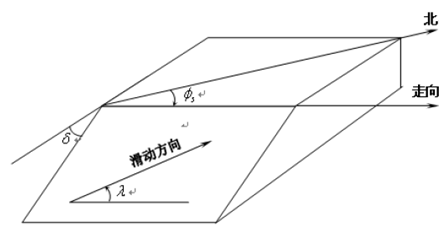
\includegraphics[width=\textwidth]{fig201.png} 
  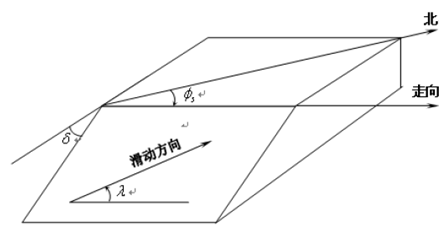
\includegraphics{fig201.png} 
  \caption{震源机制三个参数的具体意义}
  \label{fig201}
\end{figure}

\section{波形拟合反演}

\subsection{波形分解}
理论研究表明,同步地震点源\citep{Silver1982}所激发的地震波场如公式\ref{eq201}\citep{Jost1989}。
\begin{equation}
\label{eq201}
d_n(x,t)=M_{ki}[G_{nk,i}*s(t)]
\end{equation}

其中$s(t)$为震源时间函数,$Mkj$为地震矩张量,$G_{nk,i}$为格林函数,从上式可知理论波形$d$与$Mi$为线性关系。根据\citet{Kikuchi1991}的分解方法,任意地震矩张量均可由6个简单地震矩张量通过线性组合而成,如公式\ref{eq202}。
\begin{equation}
\label{eq202}
M=\sum_{k=1}^6a_kM_k
\end{equation}

公式\ref{eq202}中等式右边的$M_k$如公式\ref{eq203}所示。
\begin{equation}
\label{eq203}
\begin{array}{ccc}
M_1=\left[\begin{array}{ccc}
0 & 1 & 0\\
1 & 0 & 0\\
0 & 0 & 0\\
\end{array}\right]&
M_2=\left[\begin{array}{ccc}
1 & 0 & 0\\
0 & -1 & 0\\
0 & 0 & 0\\
\end{array}\right]&
M_3=\left[\begin{array}{ccc}
0 & 0 & 0\\
0 & 0 & 1\\
0 & 1 & 0\\
\end{array}\right]\\
M_4=\left[\begin{array}{ccc}
0 & 0 & 1\\
0 & 0 & 0\\
1 & 0 & 0\\
\end{array}\right]&
M_5=\left[\begin{array}{ccc}
-1 & 0 & 0\\
0 & 0 & 0\\
0 & 0 & 1\\
\end{array}\right]&
M_6=\left[\begin{array}{ccc}
1 & 0 & 0\\
0 & 1 & 0\\
0 & 0 & 1\\
\end{array}\right]\\
\end{array}
\end{equation}

$M_1$-$M_6$为6个简单的地震源,其中$M_6$代表爆炸源,其余5个均为剪切位错源,根据公式\ref{eq202}和公式\ref{eq203}推导可知系数a与M各分量间的对应关系如公式\ref{eq204}和公式\ref{eq205}。
\begin{equation}
\label{eq204}
M=\left[\begin{array}{ccc}
a_2-a_5+a_6 & a_1 & a_4\\
a_1 & -a_2+a_6 & a_3\\
a_4 & a_3 & a_5+a_6\\
\end{array}\right]\\
\end{equation}

\begin{equation}
\label{eq205}
\left[\begin{array}{c}
a_1\\
a_2\\
a_3\\
a_4\\
a_5\\
a_6\\
\end{array}\right]=
\left[\begin{array}{c}
M_{12}\\
(M_{11}+M_{33}-2M_{22})/3\\
M_{23}\\
M_{13}\\
(2M_{33}-M_{11}-M_{22})/3\\
(M_{11}+M_{22}+M_{33})/3\\
\end{array}\right]
\end{equation}

将公式\ref{eq202}代入公式\ref{eq201},并省略波形分量指标$n$可得到公式\ref{eq206}。
\begin{equation}
\label{eq206}
d=\sum_{k=1}^{6}a_kd_k
\end{equation}

再将公式\ref{eq205}所示的$a$与$M$关系代入公式\ref{eq206}可得到$d$关于$M$与$d_k$的公式\ref{eq207}。
\begin{equation}
\label{eq207}
\begin{array}{rl}\\
d=&M_{11}(1/3d_2-1/3d_5+1/3d_6)+M_{12}d_1+M_{13}d_4\\
&+M_{22}(-2/3d_2-1/3d_5+1/3d_6)+M_{23}d_3\\
&+M_{33}(1/3d_2+2/3d_5+1/3d_6))
\end{array}
\end{equation}

为进一步简化,将公式\ref{eq207}中$M$矩阵的6个分量依次记为 $M_1,M_2,M_3,M_4,M_5,M_6$,并将与$Mi$相乘的关于$d_k$的多项式简记为$G_i$,于是得到了简洁的6项求和的理论波形公式\ref{eq208}。在此我们按照\citet{Stein2003}专著中关于地震矩反演章节中对格林函数的推广定义,将公式\ref{eq208}中的$G_i$也称为格林函数,此格林函数即是我们之后在CPS反演中需要用到的。
\begin{equation}
\label{eq208}
d=G_iM_i(i=1,2,...6)
\end{equation}

于是任意地震矩产生的波形均可由其矩张量矩阵和6个格林函数线性叠加得到,而格林函数又可由6个已知基本地震矩激发的波形$d_k(k=1,2,...6)$叠加得到。由于以上运算均是线性运算,在$d_k$已知的情况下,在计算机中经两次迭加得到$d$速度非常快。

至此,我们已经将任意剪切位错源的波形分解为6个基本震源波形的线性叠加,而叠加的系数可由该位错源的震源机制唯一确定。现在的关键问题转化为计算6个基本震源对应的理论波形$d_k$,这可通过之后要介绍的格林函数库快速实现。

\subsection{格林函数库}

通常情况下天然地震由断层间错动造成,震源均近似纯剪切位错源。习惯上人们用破裂断层的三个角度参数——走向,倾角和滑动角来更直观地描述震源机制,地震矩张量与震源机制三个参数的对应关系如公式\ref{eq209}所示\citep{Aki1980}。
\begin{equation}
\label{eq209}
\left\{
    \begin{array}{l}
    M_{11}=-M_0(sin{\delta}cos{\lambda}sin{2\phi_s}+sin{2\delta}sin{\lambda}sin^2{\phi_s})\\
    M_{12}=M_0(sin{\delta}cos{\lambda}cos{2\phi_s}+1/2sin{2\delta}sin{\lambda}sin{2\phi_s})\\
    M_{13}=-M_0(cos{\delta}cos{\lambda}cos{\phi_s}+cos{2\delta}sin{\lambda}sin{\phi_s})\\
    M_{22}=M_0(sin{\delta}cos{\lambda}cos{2\phi_s}-sin{2\delta}sin{\lambda}cos^2{\phi_s})\\
    M_{23}=-M_0(cos{\delta}cos{\lambda}sin{\phi_s}-cos{2\delta}sin{\lambda}cos^2{\phi_s})\\
    M_{33}=M_0sin{2\delta}sin{\lambda}\\
    \end{array}
\right.
\end{equation}

其中,$\phi_s$是走向,$\delta$是倾角,$lambda$是滑动角。 $M_0$是最早由\citet{Aki1966}提出的用来度量震源长周期辐射的强度,最初称为地震矩。由于是一个标量,现在又叫作标量地震矩,代表了地震的强度。将公式\ref{eq209}代入公式\ref{eq208}即将公式转化为了理论波形关于震源机制三参数的形式。

现在我们进一步研究$d_k$如何计算,在均匀介质\citep{Ben-Menahem1963}和层状介质\citep{Haskell1964}模型的面波波场辐射理论基础上,\citet{Wang1980} 进一步得到了剪切位错源在层状速度模型中所激发的地震波场,在柱坐标频域下的表示,如公式\ref{eq210}所示。
\begin{equation}
\label{eq210}
\left\{
    \begin{array}{l}
    U_z(r,\phi,0,\omega)=Z_{SS}{\cdot}s_2+Z_{DS}{\cdot}s_3+Z_{DD}{\cdot}s_1\\
    U_r(r,\phi,0,\omega)=R_{SS}{\cdot}s_2+R_{DS}{\cdot}s_3+R_{DD}{\cdot}s_1\\
    U_{\phi}(r,\phi,0,\omega)=T_{SS}{\cdot}t_2+T_{DS}{\cdot}t_1\\
    \end{array}
\right.
\end{equation}

公式\ref{eq210}中各符号意义如\ref{eq211}所示,\ref{eq211}中$\phi$是地震观测台站相对震源的方位角,$\lambda$,$\delta$,${\phi}_s$分别代表断层滑动角,倾角,走向。公式\ref{eq210}中的$Z_{SS}$,$R_{SS}$,$T_{SS}$分别对应于$\delta=90^\circ$,$\lambda=0^\circ$的纯走滑型断裂的理论地震图的垂向、径向、切向分量;$Z_{DS}$,$R_{DS}$,$T_{DS}$分别代表$lambda=90^\circ$,$\delta=90^\circ$的纯倾滑型逆冲断层激发的地震波的垂向、径向、切向分量;$Z_{DD}$和$R_{DD}$分别对应于倾角$\delta=45^\circ$,滑动角$\lambda=90^\circ$的逆冲断层激发的理论地震波的垂向、径向分量。它们8个是合成任意剪切位错源理论地震图所需要的全部基本函数,它们是对波数K的积分表达\citep{Wang1980} 。格林函数库即由大量的不同震中距,不同震源深度对应的这8个基本函数组成。
\begin{equation}
\label{eq211}
\left\{
    \begin{array}{l}
    s_1=1/2{sin\lambda}sin{2\delta}\\
    s_2={cos\lambda}{sin\delta}sin2({\phi}-{\phi}_s)+1/2{sin\lambda}{sin2\delta}cos2({\phi}-{\phi}_s)\\
    s_3=-{cos\lambda}{cos\delta}cos({\phi}-{\phi}_s)+{sin\lambda}{cos2\delta}sin({\phi}-{\phi}_s)\\
    t_1={cos\lambda}{cos\delta}sin({\phi}-{\phi}_s)+{sin\lambda}{cos2\delta}cos({\phi}-{\phi}_s)\\
    t_2={cos\lambda}{sin\delta}cos2({\phi}-{\phi}_s)-1/2{sin\lambda}{sin2\delta}sin2({\phi}-{\phi}_s)\\
    \end{array}
\right.
\end{equation}

利用公式\ref{eq209}可推算出公式\ref{eq203}中所示6个基本地震所对应的震源机制,即各地震的3个角度参数,将其代入公式\ref{eq210},并积分变换到时间域,便得到了$d_k$,进而得到$d$。而根据公式\ref{eq211}知$s_1$、$s_2$、$s_3$、$t_1$、$t_2$等量均与$\omega$无关,结合公式\ref{eq210}可推得时间域的$Z_{SS}$,$R_{DD}$等量与$d_k$的关系也是线性的,可通过快速线性叠加得到。

综上分析知,计算$d$的关键在于得到该速度模型下,对应震中距和震源深度的$Z_{SS}$,$R_{DD}$等基本函数。而计算该函数由于要经过大量积分运算,计算速度非常慢,在迭代或搜索反演过程中实时计算一系列该基本函数是不可取的。在实际工作中通过将研究区域按一定精度格点划分,并事先计算好各格点的基本函数,并将大量的各点所对应的基本函数归档存储为格林函数库。之后理论波形数值计算需要时,直接在格林函数库中调用对应震中距和震源深度的基本函数即可,这样便实现了$d$的快速计算。经检验,这样叠加计算理论波形的速度非常快,能满足格点搜索时大量理论波形图计算的需要。

\subsection{格点搜索}

CAP与CPS方法计算波形的拟合度时使用了不同的目标函数,CAP方法先将理论波形与实测波形通过互相关运算进行时差调整,再计算调整后的波形间残差范数(L1或L2)\citep{Zhao1994},该残差范数定为为最终的目标函数,CPS方法则直接将理论与实测波形的互相关函数作为目标函数。为了单独分析权重因素对反演的影响,对比CPS与CAP不同定权的差异,后文反演试验及讨论均基于CPS的目标函数方案。CPS方法中的互相关目标函数Fit如公式\ref{eq212}定义。
\begin{equation}
\label{eq212}
Fit=(\int_{Tb}^{Te}Y(t)G(t)dt)^2/(\int_{Tb}^{Te}Y(t)Y(t)dt*\int_{Tb}^{Te}G(t)G(t)dt)
\end{equation}

在计算机中进行数值计算时使用公式\ref{eq213}所示离散形式:
\begin{equation}
\label{eq213}
Fit=[\sum_{j=1}^{N}\sum_{m-1}^{6}yg(j,m,k)M_m]^2/{[\sum_{j=1}^{N}yy(j)][\sum_{j=1}^{N}\sum_{m=1}^{6}\sum_{n=1}^{6}gg(j,m,n)M_mM_n]}
\end{equation}

公式\ref{eq213}中各符号表示的含义如公式\ref{eq214}和公式\ref{eq215}所示。
\begin{equation}
\label{eq214}
\left\{
    \begin{aligned}
    yy(j)&=\sum_{h=1}^{H(j)}y(j,h)y(j,h)wt(j)\\
    gg(j,m,n))&=\sum_{h=1}^{H(j)}g_{m}(j,h)g_{n}(j,h)wt(j)\\
    yg(j,m,k))&=\sum_{h=1}^{H(j)-|k|}\mathop{{y}'}(j,h)\mathop{{g}'_{m}}(j,h)wt(j)
    \end{aligned}
\right.
\end{equation}

\begin{equation}
\label{eq215}
\left\{
    \begin{aligned}
    \mathop{{y}'}(j,h)&=y(j,h+k) &k\geq0 \\
    \mathop{{g}'}(j,h)&=g(j,h)   &k\geq0 \\
    \mathop{{y}'}(j,h)&=y(j,h)   &k<0 \\
    \mathop{{g}'}(j,h)&=g(j,h-k) &k<0 \\
    \end{aligned}   \\
\right.
\end{equation}

N为参与反演的观测波形总道数,$H(j),wt(j)$分别为第$j(j=1,2,...N)$道波形的总采样点数及权重因子,$y(j,h),g(j,h)$分别为公式\ref{eq208}中,第$j$道观测波形$d(j)$及其对应的格林函数$Gi(j)$经过相同的数据处理(去噪等),可直接用于反演的波形的第$h(h=1,H)$个采样点,$k$为使$yg(j,m,k)$取得最大值的整数,它是Tan等\citep{Tan2006}提出的到时差平移参数,可以有效地减小系统性误差的影响。本文计算的矩震级$M_w$是由波形振幅比值计算得到的标量矩转换得到的,采用如公式\ref{eq216}所示2005年被CoSOI(Commission on Seismological Observation and Interpretation)采纳的IASPEI标准,其中$M_0$的单位为dyne-cm。
\begin{equation}
\label{eq216}
	M_w=2/3(logM_0-16.1)
\end{equation}

理论地震图可用多种方法计算,本文通过之前章节所述的用格林函数库快速合成理论波形,而格林函数库则用CPS软件包中的hprep96,hspec96,hpulse96子程序计算得到,该子程序的基本原理是波数积分法。反演时考虑到震源机制解的全空间(走向0°-360°,倾角0°-90°,滑动角-180°-180°)较小,通常采用全空间格点搜索法。

格点搜索法将全空间划分为一定精度间隔的格点,并依次遍历全部格点找寻目标函数最值点,最值处对应格点即为最优解。本文如公式\ref{eq213}所示目标函数Fit的具体计算过程如下,将遍历到的格点震源机制转换为等价地震矩张量\citep{Jost1989},同时用格林函数库快速求出公式\ref{eq208}中对应的格林函数$Gi$,将格林函数$Gi$,观测波形$d$进行必要且相同的滤波、截取时窗处理,并将处理后格林函数$g$,观测波形$y$和地震矩张量$M$与代入公式\ref{eq213},计算即可求得该格点处的拟合度Fit。


\section{数据质量影响}

\subsection{数据质量简介}

一般反演的概念是指在给定观测数据情况下,选定一个反演标准,即目标函数,如误差最小二乘标准(简称最小二乘标准),模型最小二范数标准等,然后依赖待反演模型与观测数据的理论关联公式,按选定的目标函数寻找最优的模型。具体寻找最优模型的方法称为反演方法,如线性反演方法(牛顿法,共轭梯度法等),非线性反演方法(模拟退火,遗传算法,以及本文的格点搜索方法等)。然而需要明白,在理想情况下(即不考虑计算过程中产生的各种数值误差,各算法的复杂度,理论公式的近似性,结构性系统误差等),待求模型的最终结果与反演算法是无关的,而是由反演标准和输入观测数据两者唯一决定,不同反演算法差异只是体现在寻找该最优解时的效率和准确度上。

因此,当反演标准确定的情况下(例如本文反演所使用的波形互相关拟合标准),对反演结果具有决定性的就是原始的观测数据。不同的观测数据决定了不同的反演结果,良好的观测数据对应着与真值接近的反演结果。通常我们用数据质量来描述观测数据的好坏,数据质量又可分为数据信噪比和数据结构两方面。

\subsection{数据信噪比}

顾名思义,数据信噪比代表在观测数据中,难以分离的有用信号与无用噪声的比值,是对数据真实程度的一个评价。信噪比越差,代表该数据包含的真实有用信息越少,而随机噪声对反演结果产生的不确定性干扰也可能越大。如果噪声超过了一定极限值,真实信号完全淹没在噪声中,反演结果基本由噪声决定,完全失去了参考价值,甚至产生严重的误导作用。所以实际反演时,会采用一系列办法尽量争取高信噪比输入,以保证结果的可靠性。常用的手段如高噪声数据剔除、滤波压制噪声、合理分配权重抑制强噪声数据影响等。

\subsection{数据结构}

数据结构在本文中指代数据对待求模型的约束力度,同时包括数据容量和分布状况。在反演过程中体现为观测方程对待解模型参数能否确定,较差的数据结构对应着反演中的模型欠定情况。实际反演中,观测数据的数据结构越差,对待求模型的约束效果越弱,越可能出现在同一反演标准下多解的情况,并且各解在当前反演系统下等价,无法区分。在波形反演中,为了改良数据结构,可以选用方位分布良好的台站数据作为反演输入,通过合理权重配比调整各数据在反演中的影响,以对模型参数有更强约束。

\subsection{小结}

数据信噪比和数据结构是决定数据质量的两个相对独立的方面,单纯高信噪比并不代表好的数据质量,若数据结构太差,可能导致反演时找到一系列完美符合反演标准的解,却无法分辨其中哪个解才是真实的。相反,即使信噪比稍低,但若具有同样良好的数据结构,通过反演解算即使无法找到达到完美反演标准的解,但最优解却与其它解差别比较明显,易于保证解的唯一性。

反演时,需要同时兼顾数据质量的两方面,通过数据预处理或合理的权重配比能一定程度改善数据结构。

\section{定权优化方案}

反演通常采用大量波形数据,而数据在反演中所占权重会对最终结果有决定性影响,因此合理设置$wt$值非常重要。CPS方法从数据的信噪比着手定权,考虑到信噪比随震中距增加而下降的趋势,将权重设为震中距的反比例函数,台站震中距越远的数据权重越小。CAP方法\citep{Zhu1996}则注意到波形间振幅的差异,高振幅的波形数据对反演结果起主导作用,导致低振幅波形的数据信息得不到充分利用。考虑到几何扩散是导致振幅衰减的重要原因,CAP令$wt$为震中距的幂函数,使得震中距远的台站权重相对较大,以补偿振幅的衰减。综上可知CAP和CPS方法的权重分别侧重考虑调节波形振幅和信噪比的差异。振幅调节的作用是当有振幅差异较大的多道波形参与反演时,防止强振幅的波形主导反演结果,使不同振幅的波形对反演具有相当的贡献,所以当有大量有振幅差异的波形数据参与反演时,为充分利用各道波形的信息约束反演结果必须设置振幅调节权重因子。但另一方面,振幅调节权重会进一步放大数据信噪比的差异,所以还应合理考虑信噪比定权,使高信噪比数据在反演中具有较大的影响力。基于上述分析,本文联合CPS与CAP的加权方案,将信噪比权重项$wt1$与振幅调节权重因子$wt2$的乘积设为最终的权重因子$wt$。

CPS和CAP的权重均用震中距的函数进行计算定值,这主要考虑到地震波有衰减和几何扩散效应,随着震中距增大波形的振幅会减小,从而数据信噪比也降低。但实例计算发现简单的函数难以精确描述波形振幅或信噪比与震中距的关系,本文以2013年芦山地震未经滤波处理的远场地震波数据为例,计算分析信噪比及振幅随震中距变化的情况。首先假设P波之前的噪声数据为该台站观测数据的噪声平均样本,并设其为高斯白噪声,我们分别用观测波形的标准差(WaveStd)和噪声的标准差(NoiseStd)来衡量其振幅强度,并用比值(NoiseStd/WaveStd)评估数据的相对误差。计算得到波形相对误差随震中距变化的关系如图\ref{fig202}(a)所示,可以看到相对误差随震中距变化比较散乱。为了使图像更直观展示相对误差随震中距的变化趋势,图\ref{fig202}(c)对图\ref{fig202}(a)中数据点进行最小二乘线性回归分析,将数据点进行连线并用虚线表示其回归直线,可以发现相对误差随着震中距增大而明显增加,表明信噪比确实随着震中距增大而降低。另一方面,如图\ref{fig202}(d)所示,地震波传播的几何扩散效应导致波形振幅强度随着震中距增大逐渐降低。
\begin{figure}
\centering
%  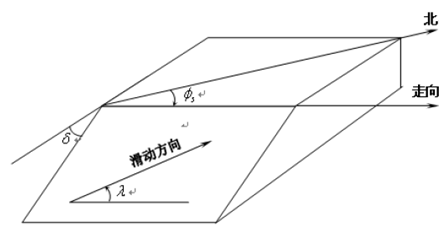
\includegraphics[width=\textwidth]{fig201.png} 
  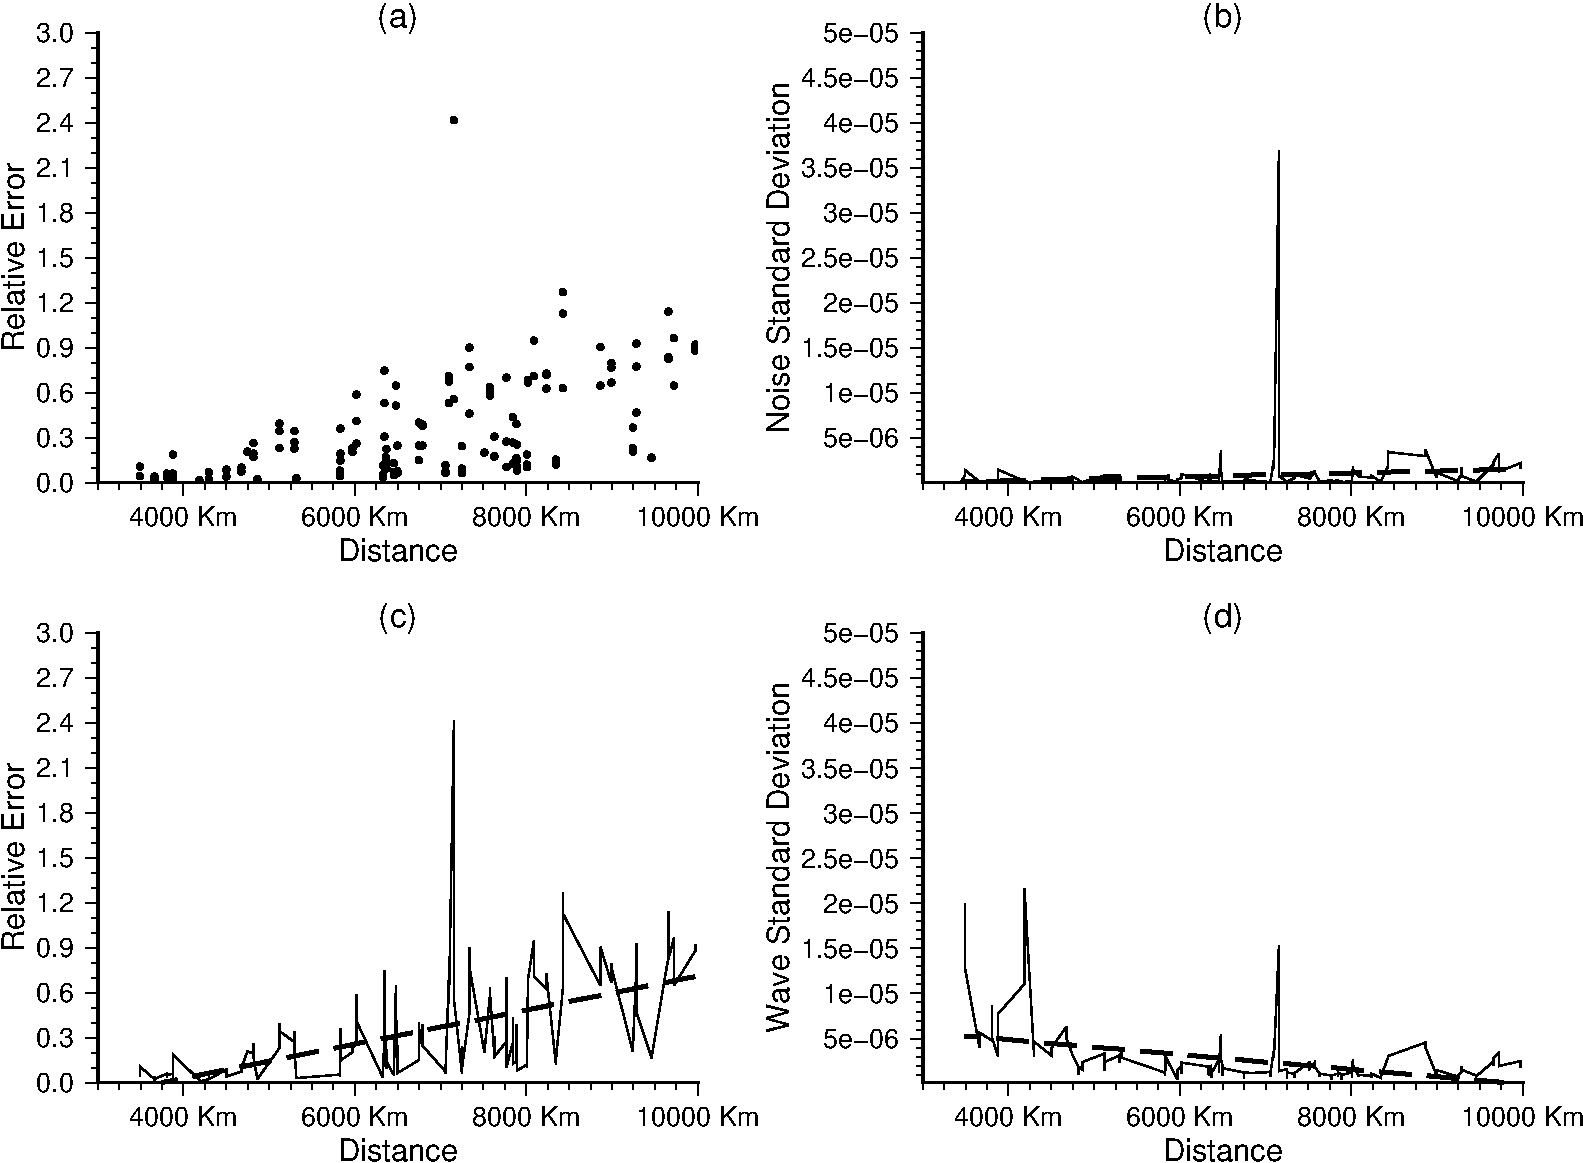
\includegraphics[scale=0.59]{fig202.pdf} 
  \caption{(a)不同震中距相对误差的分布,(b)(c)(d)分别为噪声、相对误差及波形振幅与震中距关系及统计回归线(虚线)}
  \label{fig202}
\end{figure}

虽然上述的线性回归分析表明震中距与波形的信噪比或者振幅存在一定负相关性,但从图\ref{fig202}(c)和(d)中也明显看到相对误差和波形振幅强度随着震中距单调趋势变化过程中均有着不可忽视的波动性,导致它们与震中距的关系难以用简单的初等函数进行描述。这主要是因为波形振幅不仅仅由震中距完全决定,地下浅层结构的复杂性等因素也会对振幅造成难以估计的影响,所以尽管图\ref{fig202}(b)所示的随机噪声强度随震中距变化一直较平稳,但是作为波形噪声与振幅比值的相对误差却如图\ref{fig202}(c)所示有很大的波动性。综上分析,通过震中距的函数计算得到的信噪比或振辐调节权重因子是粗糙的,此外函数的具体确定也有较强主观性,如Zhu等使用的振幅调节因子中的$r_0,p$参数的赋值可能因人而异。鉴于以上原因,本文舍弃用震中距表示权重的方法,而利用每道波形本身的数据信息直接进行针对性定权,对数据处理后的每道波形,用前文标准差比值的方法评估相对误差RelativeError,并设$|1-RelaitveError|$为信噪比权重因子$wt1$,用波形的L2范数L2norm估计平均振幅,并构造表达式$1/L2norm$作为振幅调节权重因子$wt2$,最终权重$wt$即定为$(1-NoiseStd/WaveStd)/L2norm$。

\section{误差评定方法}

实际工作中利用随机样本分析总体的统计学原理,主要分为三步。

1数据噪声评估:首先假定在台站接收特定地震事件波形的那一小段时间,台站附近的噪声是相对稳定的,且仪器接收到的噪声序列为高斯白噪声,通过对地震波到达该台站前所记录的噪声序列样本进行参数估计,便能得到各台站数据噪声的概率分布函数F(x);

2模拟数据样本:利用数据噪声的分布函数F(x)可模拟出N个随机噪声样本NOISE1,NOISE2...NOISEN,任一个噪声样本NOISEi(i=1,2,3..N)中均包含有对应于各观测台站的随机噪声,将NOISEi(i=1,2,3..N)分别加回到原始数据样本DATA0,便生成了包含合理随机噪声的N个数据样本DATA1,DATA2...DATAN;

3震源机制误差估计:利用每个数据样本DATAi(i=1,2,3...N)分别独立进行震源机制反演,可以得到误差范围内随机分布的多个震源机制M1,M2...MN,所有Mi(i=1,2,3...N)组成了一个解集样本MECH。当样本MECH容量N足够大,且包含的震源机制随机性足够好时,由统计学原理可知,样本MECH的分布可以表征原问题中震源机制的误差情况。
